\section{Search}

Our goal is to implement search algorithm based on the graph generated by our model. 
We focused on two differend algorithm: UCT (Upper Confident Bound) and ABCD (Alpha-Beta Considering Durations).  
It is well known that a good child ordering in a game tree graph can greatly improve performances.  
If better child are searched first, Alpha-Beta can produce better cuts and search deeper and UCT search will spend less time exploring less valuable moves. 
The time restriction of RTS game is transposed in term of graph exploration as a maximum number of child and/or depth limitation. 
This idea is reffered as \emph{move ordering} in \cite{portfolio}.
Their main idea behind move ordering is to consider first actions that would be produced by scripted behaviors.

\subsection{UCT Search}
UCT, or Upper Confidence bound for Trees, is the most popular Monte Carlo Tree Search algorithm for playing games that are otherwise hard for computers to handle.
This algorithm has recently seen success in the game of go, but more relevant to our topic, also been applied to games such as Arimaa, and even RTS games. For a review of how it works we refer to \cite{mcts}.
Arimaa is interesting because it has an average branching factor of 17000, compared to chess, which only has 35. \cite{arimaawiki}

In \cite{wargusuct}, UCT is used for deciding where squads should attack in the RTS game Wargus, which would correspond to using UCT at the General-level in our conceptual model as well.

\subsection{ABCD Search}
In \cite{abcd}, an extended version of alpha-beta pruning, which is also a searching algorithm, was used for micro-management. 
They were able to find good solutions for 8 v.s. 8 unit scenarios in 5 ms, achieving around a 80\% win rate against their best script.

The evaluation functions suggested by \cite{abcd} are the following:
\begin{shortitem}
\item Straight Forward Evaluations:
$$
    \displaystyle{SFE(s) = \sum_{u \in U_1} u.hp - \sum_{u \in U_2} u.hp } 
$$

\item Life Time Damage:
$$
    \displaystyle{LTD(s) = \sum_{u \in U_1} u.hp \cdot u.DPF- \sum_{u \in U_2} u.hp \cdot u.DPF } 
$$

\item Life Time Damage 2:
$$
    \displaystyle{LTD2(s) = \sum_{u \in U_1} \sqrt{u.hp} \cdot u.DPF - \sum_{u \in U_2} \sqrt{u.hp} \cdot u.DPF } 
$$
\end{shortitem}

Where $DPF$ in the damage per frame of a unit (see section \ref{kiting}), $U_1$ (resp. $U_2$) is the set of player's (resp. opponent's) units .

$SFE$ doesn't take into account unit strike force -- which is an essential information during a battle. 
$LFD$ present a good estimation of this strike force but do not favour having a greater number of units. 
Ultimately $LTD2$ measure the strike force and favor the greatest number of units remaining. 
(Having two units with $50$ hit points gives more power than one with $100$ hit points.)

In order to use alpha-beta algorithm it is necessary to separates the player's actions and its opponents action.
It can be done quiet efficiently by considering the children of a node as the restriction of its children to only one player set of actions:
$$
S_{A|p} = \{A \in S_A | \forall a \in A, a \text{ is an action performed by $p$}\}
$$
Algorithm \ref{algABCD} presents the ABCD algorithm.
The main disctinction with the ``classic'' alpha-beta algorithm is that there is not a perfect alternation between $MAX$ and $MIN$. Once a state has no possible actions, we move in time until an action can be performed for one of the player. 
Figure \ref{figABCD} shows an exemple of such a graph: once we've reached a state where no action can be made for both player, we advance in time. In this new frame, there is an action for $MAX$. Therefore is still him who is considered as the current player.

\begin{figure}[h!t]
    \begin{algorithm}[ABCD (Alpha-Beta Considering Durations)]
        Let $s_0$ be the root node, $MAX$ be the player and $MIN$ the opponent. 
        The algorithm return the best move compute by $ABCD(s_0,d_{max},-\infty,+\infty,MAX)$ where: \ \\

        \textbf{Function} $ABCD(s,d,\alpha,\beta,p)$:
        \begin{enum}
        \item \textbf{If} ($s$ is a terminal state) \textbf{Return} $LTD2(s)$
        \item \textbf{Else}
            \begin{enum}
            \item If $S_{A|p} \neq \emptyset$ 

            \begin{enum}
            \item \textbf{While} $S_{A|p} \neq \emptyset$
                \begin{enum}
                \item Pop $s_1$ from $S_{A|p}$ 
                \item Let $v = ABCD(s_1,d-1,\alpha,\beta,\bar{p})$
                \item \textbf{If} $p = MAX$ and $(v > \alpha)$ \textbf{then} $\alpha = v$
                \item \textbf{If} $p = MIN$ and $(v < \beta)$ \textbf{then} $\beta= v$
                \item \textbf{If} $\alpha \geq \beta$ \textbf{then break} 
                \end{enum}
            \item \textbf{Return} $(p = MAX) ? \alpha : \beta$ 
            \end{enum}
        \item \textbf{Else if} $S_{A|\bar{p}} \neq \emptyset$
            \begin{enum}
            \item \textbf{Return} $ABCD(s,d,\alpha,\beta,\bar{p})$
            \end{enum}
        \item \textbf{Else} 
            \begin{enum}
            \item Advance in time to state $s'$ for which $S'_A \neq \emptyset$
            \item \textbf{Return} $ABCD(s',d,\alpha,\beta,p)$
            \end{enum}
        \end{enum}
        \end{enum}
        \ \\
        And $s$ being considered as a \textbf{terminal state} if $d_{max}$ is reached, the time is elapsed or the state is a winning/loosing situation.
        \label{algABCD}
    \end{algorithm}
\end{figure}

\begin{figure}[h!t]
\centering
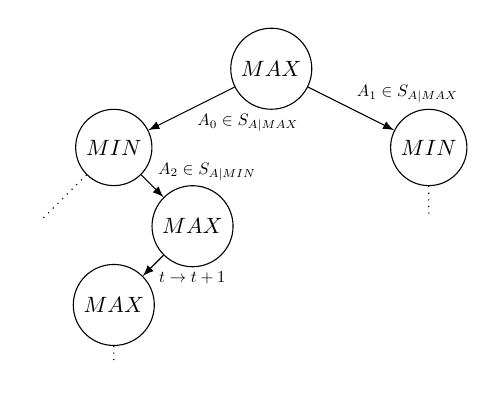
\begin{tikzpicture}[node distance = 1cm]
    \tikzstyle{node}=[circle,align=center,scale=0.8,draw]
    \tikzstyle{nodenotgen}=[circle,dotted,align=center,scale=0.8,draw]
    \tikzstyle{nodeterm}=[circle,fill=gray!30,align=center,scale=0.8,draw]
    \tikzstyle{link}=[->,thin,>=latex]
    
    \node[node] (s0) at (4,4) {$MAX$};

    \node[node] (s1) at (2,3) {$MIN$};
    \node[node] (s3) at (6,3) {$MIN$};

    \node[auto,scale=0.8] (s33) at (6,2) {};
    \draw[-,>=latex,dotted] (s3) to (s33);

    \node[auto,scale=0.8] (s4) at (1,2) {};
    \node[node] (s6) at (3,2) {$MAX$};

    \node[node] (s7) at (2,1) {$MAX$};

    \node[auto,scale=0.8] (s8) at (2,0.2) {};
    
    \draw[link] (s0) to node [auto,scale=0.6] {$A_0 \in S_{A|MAX}$} (s1); 
    \draw[link] (s0) to node [auto,scale=0.6] {$A_1 \in S_{A|MAX}$} (s3);
    \draw[-,>=latex,dotted] (s1) to (s4);
    \draw[link] (s1) to node [auto,scale=0.6] {$A_2 \in S_{A|MIN}$} (s6);
    \draw[link] (s6) to node [auto,scale=0.6] {$t \rightarrow t+1$} (s7);
    \draw[-,>=latex,dotted] (s7) to (s8);
    

\end{tikzpicture}
    \caption{Exemple of a graph constructed by the ABCD-algorithm}
    \label{figABCD}
\end{figure}
